\documentclass{article}
\usepackage{amsmath, amssymb, amsthm, array, fancyhdr, graphicx, enumerate, enumitem, stackengine}
\usepackage[margin = 1in]{geometry}

\def\class{Math 338}
\def\header{Project II - Categorical Variables}
\def\first{Jason}
\def\last{Wong}

\graphicspath{ {./img/} }

\fancypagestyle{useheader}
{
  \fancyhf{}
  \setlength{\headsep}{\baselineskip}
  \lhead{\class}
  \chead{\header}
  \rhead{\last, \first}
  \cfoot{\thepage}
}

% logical operators
\let\iff\leftrightarrow
\let\lnot\neg
\let\xor\oplus


% floor function
\newcommand{\floor}[1]{\lfloor #1 \rfloor}


% draws a black square for proofs
\renewcommand{\qed}{\hfill$\blacksquare$}

\newcommand{\solution}[1]{
  \textbf{Solution} #1
}

\newcommand{\step}[1]{
  \begin{enumerate}
    \item[{}] #1
  \end{enumerate}
}

% args: (equation (aligns at & sign: x &= y), explanation)
\newcommand{\proofstep}[2]{&#1 &&\ \  \text{#2}}

% args: (number, question, steps, explanation)
\newenvironment{twocolproof}[1]{
    \begin{align}
      #1
    \end{align}
    \setcounter{equation}{0}
}

% args (number, problems, subproblemss)
\newenvironment{nestedproblem}[3]{
  \begin{enumerate}
    \item[\bfseries{#1}] #2
    #3
  \end{enumerate}
  \hfill
}

% args: (number, question, solution)
\newenvironment{problem}[3]{
  \begin{enumerate}
    \item[\bfseries{#1}] #2
    \begin{enumerate}
      \item[{}] #3
    \end{enumerate}
  \end{enumerate}
  \hfill
}

\begin{document}
\pagestyle{useheader}
  \begin{problem}{1}{Perform a Goodness-of-Fit test and see if the data supports that the personality roles are not randomly assigned.}{
    \begin{tabular}{ |c|c|c|c|c| } 
      \hline
      Personality Role & Observed Count & Expected Count & Observed Count & Expected Proportion\\ 
      \hline
      Analysts & 35 & 23 & 0.38043 & 0.25\\
      Diplomats & 26 & 23 & 0.28261 & 0.25\\
      Explorers & 16 & 23 & 0.17391 & 0.25\\
      Sentinels & 15 & 23 & 0.16304 & 0.25\\
      \hline
    \end{tabular}
    \linebreak
    \linebreak
    $H_0:$ The distribution of personalities are equal\\
    $H_a:$ The distribution of personalities are not equal\\
    $$df = 3$$
    $$\chi^2 = \sum \frac{(Observed - Expected)^2}{Expected} = 11.5652$$
    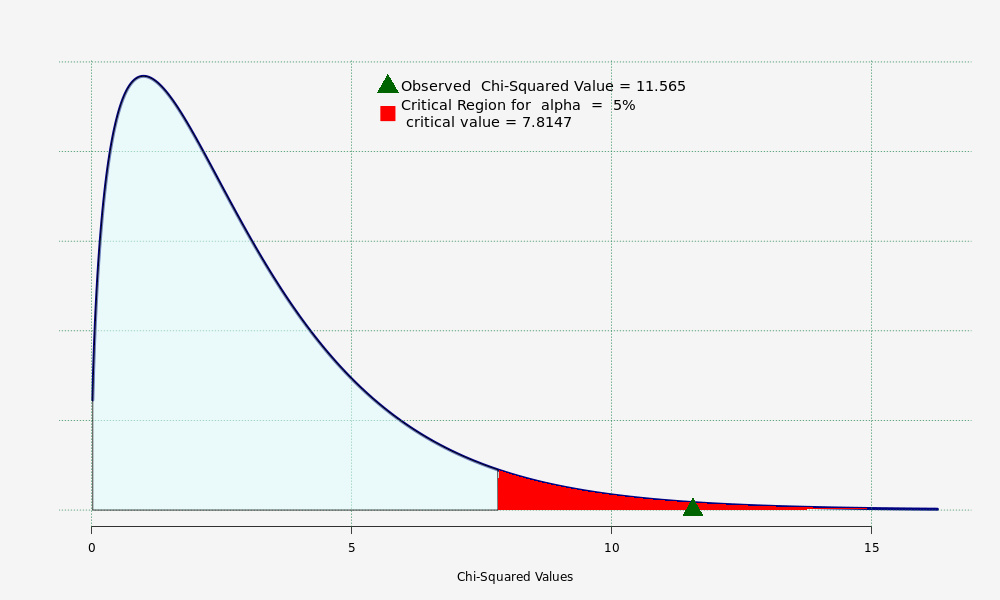
\includegraphics[scale=0.42]{1}
    \linebreak
    \linebreak
    Conclusion: Because our $\chi^2$ value is greater than the critical value at a 5\% significance level, we reject the null hypothesis the that the distribution of personality types are equal and accept the alternative that concludes that personalities are not randomly assigned 
  }
  \pagebreak
  \end{problem}
  \begin{problem}{2}{Test if the personality role and one of the other categorical variables (your choice: College) are independent.}{
    \textbf{Observed}\\
    \begin{tabular}{ |c|c|c|c|c|c| } 
      \hline
      College & Analysts & Diplomats & Explorers & Sentinels & \textbf{Total}\\ 
      \hline
      College X & 1 & 1 & 0 & 0 & 2\\
      College Y & 1 & 0 & 0 & 0 & 1\\
      College Z & 0 & 1 & 0 & 0 & 1\\
      Engineering and Computer Science & 22 & 14 & 12 & 10 & 58\\
      Natural Sciences and Mathematics & 11 & 10 & 4 & 5 & 30\\
      \hline
      \textbf{Total} & \textbf{35} & \textbf{26} & \textbf{16} & \textbf{15} & \textbf{92}\\
      \hline
     \end{tabular}\\\\
    \textbf{Expected}\\
    \begin{tabular}{ |c|c|c|c|c|c| } 
      \hline
      College & Analysts & Diplomats & Explorers & Sentinels & \textbf{Total}\\ 
      \hline
      College X & 0.76 & 0.57 & 0.35 & 0.33 & 2\\
      College Y & 0.38 & 0.28 & 0.17 & 0.16 & 1\\
      College Z & 0.38 & 0.28 & 0.17 & 0.16 & 1\\
      Engineering and Computer Science & 22.07 & 16.39 & 10.09 & 9.46 & 58\\
      Natural Sciences and Mathematics & 11.41 & 8.48 & 5.22 & 4.89 & 30\\
      \hline
      \textbf{Total} & \textbf{35} & \textbf{26} & \textbf{16} & \textbf{15} & \textbf{92}\\
      \hline
    \end{tabular}
    \linebreak
    \linebreak
    $H_0:$ Personality type and College are independent\\
    $H_a:$ Personality type and College are not independent\\
    $$df = (Rows - 1)(Columns - 1) = (5 - 1)(4 - 1) = 12$$
    $$\chi^2 = \sum \frac{(Observed - Expected)^2}{Expected} =6.5682$$
    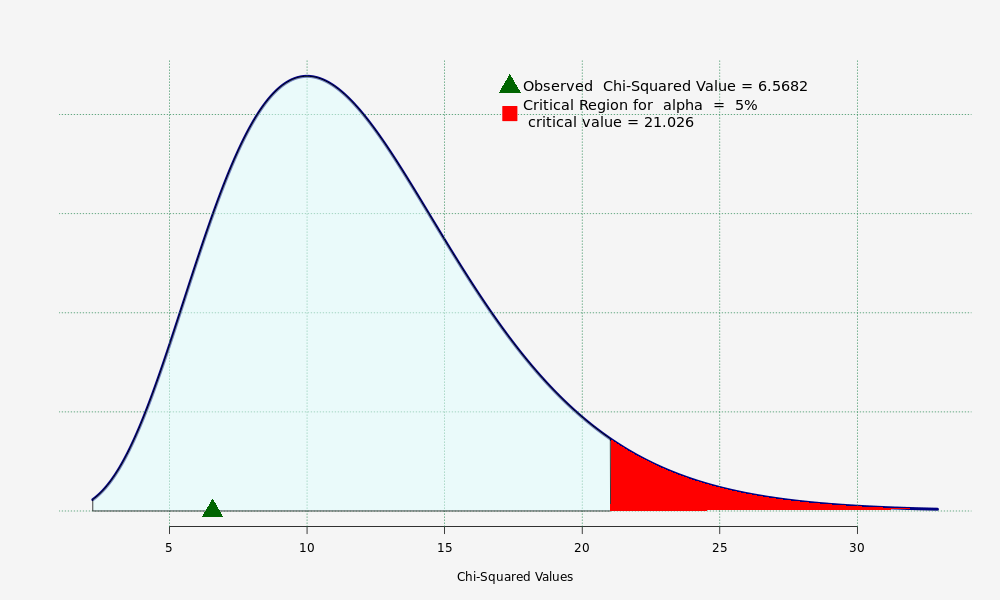
\includegraphics[scale=0.42]{2}\\
    Conclusion: Because our $\chi^2$ value is less than our critical value at a 5\% significance level, we fail to reject the null hypothesis and we can conclude that personality type and college are independent.
  }
  \end{problem}
\end{document}